\input{../header}
\hyphenpenalty=5000

\usepackage{pgfplots}
\pgfplotsset{compat=1.5}

\rhead{Your name: \rule{8cm}{0.15mm}}

\begin{document}

\everymath{\displaystyle}

\section{Learning target D3, version 1}

D3: Apply Euler's Method to generate an approximate solution to an initial value problem, and explain the result's meaning in context.

\hrulefill

A population of flamingos changes over time according to the differential equation 
\[\dfrac{dP}{dt} = -\frac{1}{3}\, P\, (1-P)(5-P),\]
where $P$ is measured in thousands (and $t$ is probably measured in months or years).

\begin{enumerate}[(a), leftmargin=0pt]
	\item If $P(0) = 0.5$, use Euler's method with 3 steps to approximate $P(2)$. Record your work in a table.\\
	(Hint: If you're using 3 steps to get from $t=0$ to $t=2$, how big should $\Delta t$ be?)
	\vfill
	\item Same thing, but this time, start with $P(0) = 1.5$.
	\vfill
	\item Compare your numerical results here with your graphical results on the D2 part of this problem. What recommendations do you have for flamingo keepers?
\end{enumerate}

%%%%%%%%%%%%%%%%%%%%%%%%%%%%%%%%%%%%%%%%%%%%%%%%%%%%%%%
\pagebreak
%%%%%%%%%%%%%%%%%%%%%%%%%%%%%%%%%%%%%%%%%%%%%%%%%%%%%%%

\section{Learning target D3, version 2}

D3: Apply Euler's Method to generate an approximate solution to an initial value problem, and explain the result's meaning in context.

\hrulefill

Consider the differential equation \[\frac{dy}{dx} = -\frac{x}{y}\]

Starting with the initial condition $y(1)=1$, use Euler's method with a step size of $\Delta x = 0.25$ to find out approximately when the solution $y(x)$ would cross over the $x$-axis.

\vfill

Plot your points as you calculate them:
\begin{center}
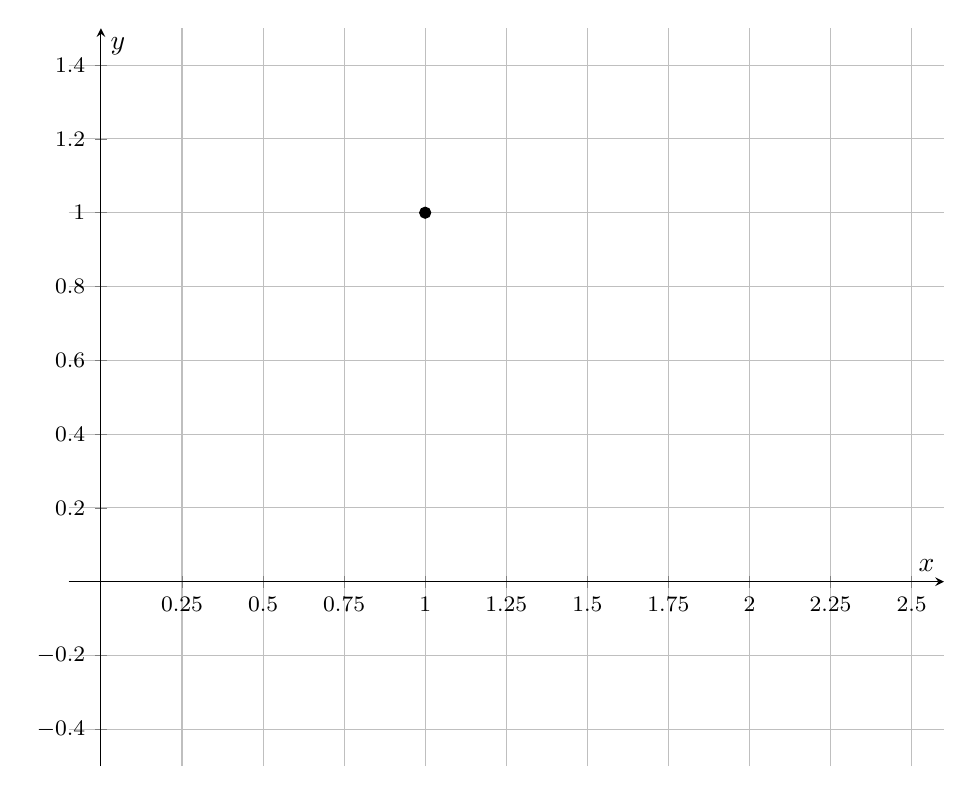
\begin{tikzpicture}
	\begin{axis}[width=5in,
		grid=major,
		xlabel = $x$, ylabel = $y$,
		tick label style={font=\footnotesize},
		xtick distance = 0.25,
		%ytick = {-3,...,3},
		xmin = -0.1, xmax = 2.6,
		ymin = -0.5, ymax = 1.5,
		axis x line = middle,
		axis y line = middle,
		grid=both,
		]
    \addplot[mark=*] coordinates{(1,1)};
	\end{axis}
\end{tikzpicture}
\end{center}

\end{document}